\documentclass[notes,slidesec,a4]{seminar}
\usepackage[spanish]{babel}
\usepackage[utf8]{inputenc}

\usepackage{t-gsyc-6}
\usepackage{fancybox}
\usepackage{graphics}
\usepackage{moreverb}
\usepackage{alltt}
\usepackage{html}
\usepackage{hthtml}
\usepackage{amsmath}
\usepackage[normalsize]{subfigure}
\usepackage{url}
\usepackage{listings}

\usepackage{eurosym}

\title{Odometría visual con sensor RGBD en JdeRobot}
\author{Javier Benito Díaz}

\cop{Javier Benito Díaz}
\address{jbenito.dz@gmail.es}

\begin{document}
\maketitle

%%--------------------------------------------------------------

\begin{hslide}
	\slsect{Índice}
	\begin{itemize}
		\item Introducción 
		\item Objetivos
		\item Infraestructura
		\item Desarrollo
		\item Experimentos
		\item Conclusiones
	\end{itemize}
\end{hslide}

%%--------------------------------------------------------------

%%--------------------------------------------------------------3
\begin{hslide}
	\slsect{Introducción}
	\slsubsect{Autolocalización visual}
	\begin{minipage}{6cm}
		\begin{center}
			\begin{figure}
				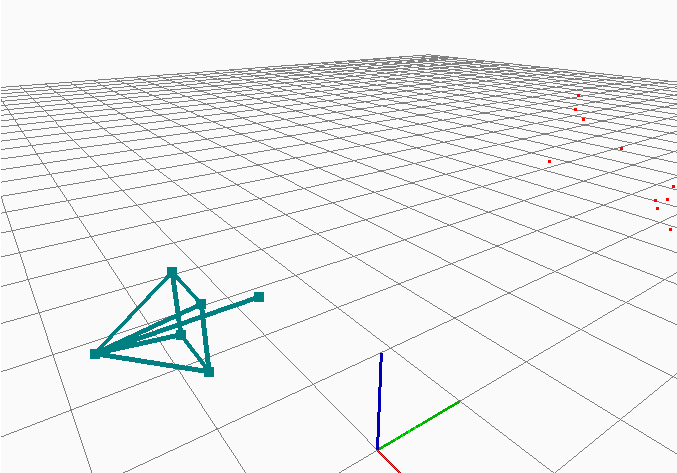
\includegraphics[width=6.0cm]{img/camera-opengl.png}
			\end{figure}
		\end{center}
	\end{minipage} \hfill
	\begin{minipage}{6cm}
		\begin{itemize}
			\item Estimar posición de una cámara
			\item 
		\end{itemize}
	\end{minipage}
\end{hslide}

%%--------------------------------------------------------------

\begin{hslide}
	\slsect{Introducción}
	\slsubsect{Visión artificial}
	\begin{minipage}{5cm}
		\begin{itemize}
			\item 
			\item 
		\end{itemize}
	\end{minipage} \hfill
	\begin{minipage}{6cm}
		\begin{center}
			\begin{figure}
				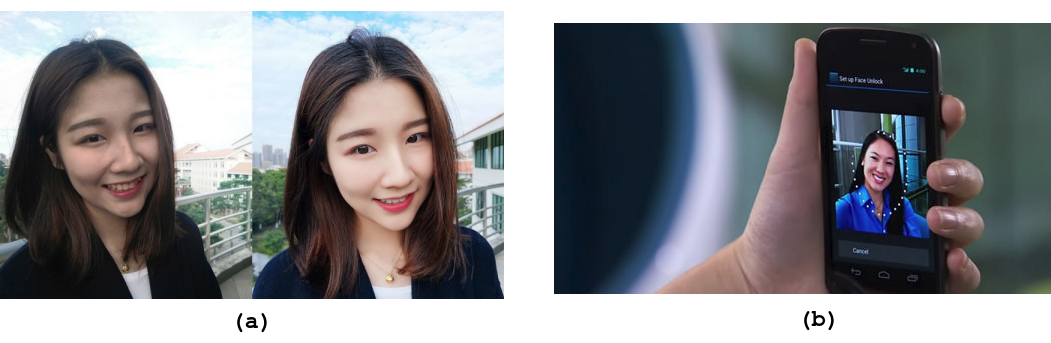
\includegraphics[width=6.0cm]{img/face.png}
			\end{figure}
		\end{center}

	\end{minipage}
\end{hslide}

%%--------------------------------------------------------------


\end{document}